\documentclass{article}
\usepackage[utf8]{inputenc}
\usepackage{tikz}
\usepackage{circuitikz}
\usepackage{hyperref}
\usepackage{float}
\usepackage{graphicx}

\usepackage{geometry}
\geometry{
a4paper,
top = 20mm,
bottom = 20mm,
left = 15mm,
right = 15mm,
}

\usepackage{parskip}
\setlength{\parindent}{0cm}

\title{IPT Summer Workshop Project Overview}
\author{2021 Summer Workshop Teams}
\date{December 2021}

\newcommand{\bd}{\textbf} % Bold 
\newcommand{\txt}{\textrm} % Text inside math mode. 
\newcommand{\subtxt}[1]{\textrm{\tiny{#1}}} % For subscript texts.

\begin{document}
    \maketitle

    \section{Introduction}
    In this project, the hardware and firmware required for the running of an RC car on a track using inductive power transfer (IPT) 
    technology. The RC car used is the \href{https://www.rchobbies.co.nz/tamiya-1-10-tt-02-subaru-impreza-monte-carlo-99-rc-car/}
    {TAMIYA 1/10 TT-02 SUBARU IMPREZA MONTE CARLO '99 RC CAR}. 

    \section{Track}
    The track will have a length $l$ and width $w$ as shown in Figure~\ref{track_top_view}. 
    \begin{figure}[H]
        \centering 
        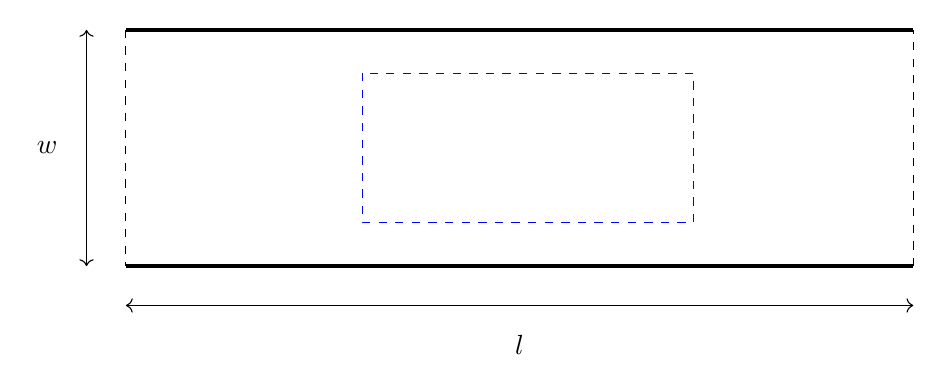
\begin{tikzpicture}
            \draw[ultra thick](0,0) to ++(10,0) coordinate(A);
            \draw[dashed](A) to ++(0,3) coordinate(B);
            \draw[ultra thick](B) to ++(-10,0) coordinate(C);
            \draw[dashed](C) to ++(0,-3);  

            \draw[<->] (-0.5, 0) to ++(0,3); 
            \node at (-1,1.5) {$w$}; 

            \draw[<->] (0,-0.5) to ++(10,0); 
            \node at (5,-1) {$l$}; 

            \draw[blue, dashed] (3,2.45) rectangle (7.21,0.55); 
            % \draw[dashed, red] (0,1.5) ++(10,0); 

        \end{tikzpicture}
        \caption{Simplified sketch of track top view; blue dashed rectangle represents car.}\label{track_top_view}
    \end{figure}
    % Add a diagram showing what the tolerance means in our case. 

    For this project, the specifications are: 
    \begin{itemize}
        \item $l > 1000\rm mm$. 
        \item $w = 300\rm mm$. 
        \item Tolerance of car alignment: $\pm 50\rm mm$. 
    \end{itemize}

    \section{System diagrams}
    Our design can be partitioned into three main sections: 
    \begin{enumerate}
        \item The primary side. 
        \item The secondary (pick-up) side. 
        \item The motor driver. 
    \end{enumerate}

    \subsection{Primary side}
    \begin{figure}[H]
        \centering 
        \begin{circuitikz}[american]
            \node[fourport, scale = 2, t = (1)] (fullbridge) at (0,0){};
            \node[fourport, scale = 2, t = (2)] (compensation) at (5,0){}; 

            \draw(fullbridge.1) to[short] ++ (-2,0) node[ground] (gnd){};
            \draw(fullbridge.4) to[short] ++ (-2,0) to[V, l = $V_{\subtxt{IN}}$] (gnd);
            \draw(fullbridge.3) to[short] (compensation.4); 
            \draw(fullbridge.2) to[short] (compensation.1); 
            \draw(compensation.2) to[short] ++ (2,0) coordinate (A);
            \draw(compensation.3) to[short] ++ (2,0) to[L, l = $L_1$] (A);

        \end{circuitikz}
        \caption{System diagram for the primary side}\label{primary_sys_diagram}
    \end{figure}

    Figure~\ref{primary_sys_diagram} outlines the hardware of our primary side. A DC voltage $30\txt{V}\leq V_{\subtxt{IN}}\leq 45\rm V$ 
    is used as the input. As we must have AC for IPT to work\footnotemark, a \bd{full-bridge inverter} (1) transforms the DC voltage 
    to a high-frequency AC voltage. An \bd{LCL} compensation network (2) with partial series compensation follows it. 
    $L_1$ is the primary coil. 

    \footnotetext{As a changing current is required for a changing magnetic flux in the primary coil $L_1$, a DC 
    current will not cause any changing flux and hence voltage induced in the secondary. Only AC will suffice.}

    \subsection{Secondary side}
    Unlike the primary, the secondary will use \bd{parallel} compensation via the capacitor $C_{st}$. A rectifier followed 
    by a voltage regulator (1) % Check this with others later. Are we using a voltage regulator?  
    generates a DC voltage which is stepped up to $V_{\subtxt{OUT}}$ via a \bd{boost converter} (4). 
    $V_{\subtxt{OUT}}$ is optimally 10V\footnotemark~but can drop as low as 4V depending on the alignment of the car 
    with the center of the track. 

    \footnotetext{This is because the car's operating voltage is 10V. It can be operated down to 4V but it will 
    have inferior performance.}
    % Maybe add (hand-drawn) diagram about alignment here or in the section about the track later. 

    \begin{figure}[H]
        \centering 
        \begin{circuitikz}[american]
            \node[fourport, scale = 2, t = (3)] (reg) at (0,0){};
            \node[fourport, scale = 2, t = (4)] (boost) at (5,0){}; 

            \draw(reg.1) to[short] ++ (-2,0) node[ground] (gnd){};
            \draw(reg.4) to[short] ++ (-2,0) coordinate (C) to[C, l = $C_{st}$, *-*] (gnd);
            \draw(C) to[short] ++ (-2,0) coordinate (D);
            \draw(gnd) to[short] ++ (-2,0) to[L, l = $L_2$] (D);

            \draw(reg.3) to[short] (boost.4); 
            \draw(reg.2) to[short] (boost.1); 
            \draw(boost.2) to[short] ++ (2,0) coordinate (A);
            \draw(boost.3) to[short] ++ (2,0) to[open, v = $V_{\subtxt{OUT}}$, o-o] (A);

        \end{circuitikz}
        \caption{System diagram for the secondary side}\label{secondary_sys_diagram}
    \end{figure}

    \subsection{Motor driver}
    A pulse-width modulated (PWM) signal $v_{\subtxt{PWM}}$ used to drive the motor is produced via 
    a full-bridge inverter (5)\footnotemark. Depending 
    on its duty cycle, the average power delivered to the motor will vary accordingly. 

    \footnotetext{The microcontroller and hence firmware play a major role in this.}
    \begin{figure}[H]
        \centering 
        \begin{circuitikz}[american]
            \node[fourport, scale = 2, t = (5)] (fullbridge) at (0,0){};

            \draw(fullbridge.4) to[short] ++ (-2,0) coordinate (A); 
            \draw(fullbridge.1) to[short] ++ (-2,0) coordinate (B);
            \draw(A) to[open, v = $V_{\subtxt{OUT}}$, o-o] (B); 
            
            \draw(fullbridge.3) to[short] ++ (2,0) coordinate (C);
            \draw(fullbridge.2) to[short] ++ (2,0) coordinate (D);
            \draw(C) to[open, v = $v_{\subtxt{PWM}}$, *-*] (D); 

            \draw(C) to[short] ++ (2,0) coordinate (E);
            \draw(D) to[short] ++ (2,0) coordinate (F);
            \draw(E) to[twoport, t = Motor] (F); 

        \end{circuitikz}
    \end{figure} 

\end{document}